\documentclass[tikz,border=5pt]{standalone}
\usetikzlibrary{positioning}
\usepackage{amsmath, amssymb}
\begin{document}
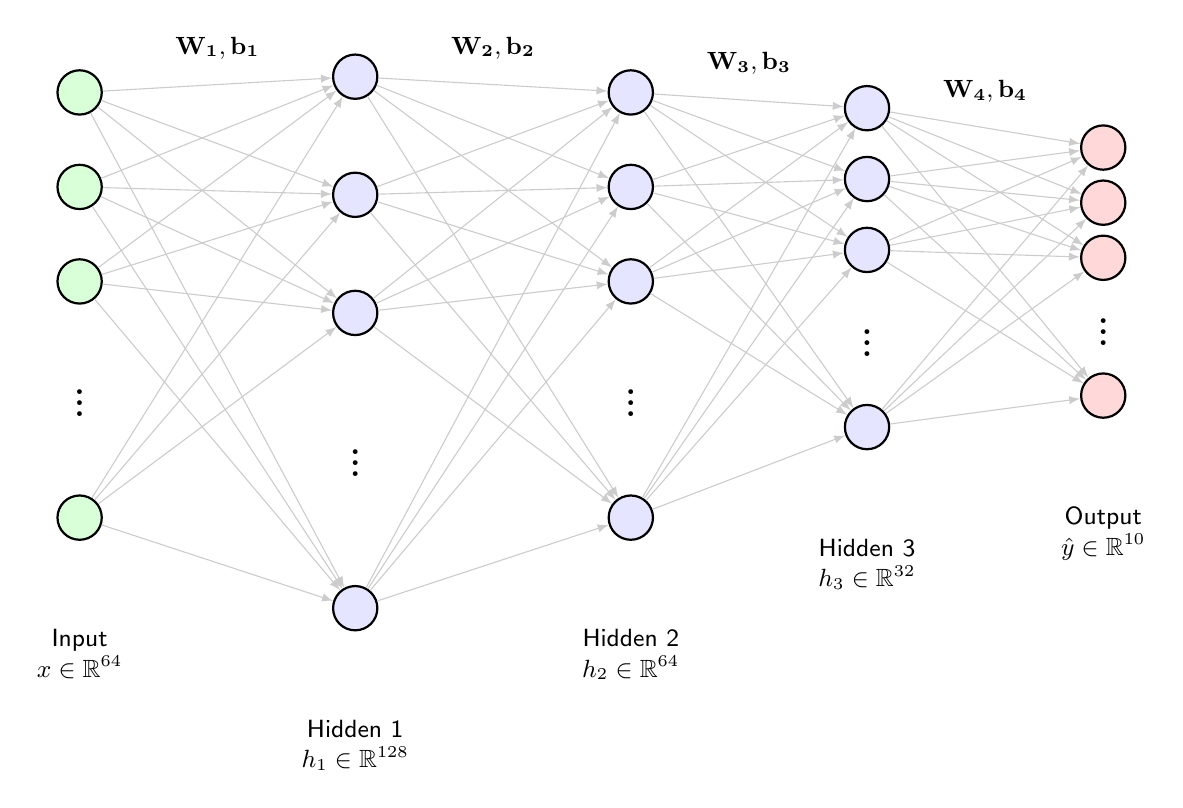
\begin{tikzpicture}[
    scale=1,
    neuron/.style={circle, draw, minimum size=16pt, inner sep=0pt, line width=0.8pt},
    input/.style={neuron, fill=green!15},
    hidden/.style={neuron, fill=blue!10},
    output/.style={neuron, fill=red!15},
    connect/.style={-latex, thin, gray!40},
    dots/.style={font=\large\bfseries},
    layer_label/.style={font=\small\sffamily, align=center, node distance=0.5cm}
]

    % --- LAYER CONFIGURATION ---
    % We define the x-position and a vertical "spread" factor for each layer
    % Input (64), H1 (128), H2 (64), H3 (32), Output (10)

    % --- LAYER 0: Input (Spread: 1.2) ---
    \foreach \i in {1,2,3} \node[input] (L0-\i) at (0, -1.2*\i) {};
    \node[dots] (L0-dots) at (0, -1.2*4.2) {$\vdots$};
    \node[input] (L0-4) at (0, -1.2*5.5) {};
    \node[below=of L0-4, layer_label] {Input \\ $x \in \mathbb{R}^{64}$};

    % --- LAYER 1: Hidden 1 (Spread: 1.5) ---
    % Spread is larger because this is the 128-node layer
    \foreach \i in {1,2,3} \node[hidden] (L1-\i) at (3.5, -1.5*\i + 0.5) {};
    \node[dots] (L1-dots) at (3.5, -1.5*4.2 + 0.5) {$\vdots$};
    \node[hidden] (L1-4) at (3.5, -1.5*5.5 + 0.5) {};
    \node[below=of L1-4, layer_label] {Hidden 1 \\ $h_1 \in \mathbb{R}^{128}$};

    % --- LAYER 2: Hidden 2 (Spread: 1.2) ---
    \foreach \i in {1,2,3} \node[hidden] (L2-\i) at (7, -1.2*\i) {};
    \node[dots] (L2-dots) at (7, -1.2*4.2) {$\vdots$};
    \node[hidden] (L2-4) at (7, -1.2*5.5) {};
    \node[below=of L2-4, layer_label] {Hidden 2 \\ $h_2 \in \mathbb{R}^{64}$};

    % --- LAYER 3: Hidden 3 (Spread: 0.9) ---
    % Spread is smaller for 32 nodes
    \foreach \i in {1,2,3} \node[hidden] (L3-\i) at (10, -0.9*\i - 0.5) {};
    \node[dots] (L3-dots) at (10, -0.9*4.2 - 0.5) {$\vdots$};
    \node[hidden] (L3-4) at (10, -0.9*5.5 - 0.5) {};
    \node[below=of L3-4, layer_label] {Hidden 3 \\ $h_3 \in \mathbb{R}^{32}$};

    % --- LAYER 4: Output (Spread: 0.7) ---
    % Tiniest spread for 10 nodes
    \foreach \i in {1,2,3} \node[output] (L4-\i) at (13, -0.7*\i - 1.2) {};
    \node[dots] (L4-dots) at (13, -0.7*4.2 - 1.2) {$\vdots$};
    \node[output] (L4-4) at (13, -0.7*5.5 - 1.2) {};
    \node[below=of L4-4, layer_label] {Output \\ $\hat{y} \in \mathbb{R}^{10}$};

    % --- DRAW CONNECTIONS & LABELS ---
    \foreach \sourceLayer / \destLayer / \labelName in {0/1/W_1, 1/2/W_2, 2/3/W_3, 3/4/W_4} {
        \foreach \i in {1,2,3,4} {
            \foreach \j in {1,2,3,4} {
                \draw[connect] (L\sourceLayer-\i) -- (L\destLayer-\j);
            }
        }
        % Math Labels positioned relative to the first nodes of each layer
        \path (L\sourceLayer-1) -- (L\destLayer-1) node [midway, above=0.2cm, font=\small] {$\mathbf{\labelName}, \mathbf{b_{\destLayer}}$};
    }

\end{tikzpicture}
\end{document}